\RequirePackage[T1]{fontenc}
\documentclass[10pt,conference,compsocconf]{IEEEtran}
\usepackage{amsmath,booktabs,graphicx,hyperref}
\hypersetup{colorlinks=true,urlcolor=blue,citecolor=blue,linkcolor=black}
% Generated from saved measurements by build_report.py
\newcommand{\HoldFone}{0.4225}
\newcommand{\HoldAccuracy}{0.8685}
\newcommand{\HoldRecall}{0.5446}
\newcommand{\HoldBalanced}{0.7223}
\newcommand{\HoldPrecision}{0.3451}
\newcommand{\CVMean}{0.4310}
\newcommand{\CVStd}{0.0004}
\newcommand{\ModelRows}{
Majority & --- & 0.9117 & 0.0000 & 0.0000\\
Linear regression & 0.22 & 0.8653 & 0.4057 & 0.5208\\
Ridge ($10^{-3}$) & 0.22 & 0.8666 & 0.4049 & 0.5141\\
Logistic, mean fill & 0.21 & 0.8724 & 0.4133 & 0.5089\\
Categorical, no L2 & 0.21 & 0.8763 & 0.4327 & 0.5343\\
Selected L2 logistic & 0.20 & 0.8722 & 0.4321 & 0.5506\\
}
\newcommand{\AblationRows}{
Mean fill + scaling & 0.4129 & ---\\
Median fill & 0.4131 & +0.0002\\
+ Missing indicators & 0.4139 & +0.0008\\
+ Categorical encoding & 0.4285 & +0.0147\\
L2 $10^{-3}\to10^{-4}$ & 0.4321 & +0.0036\\
}

\begin{document}
\title{Categorical Encoding and Threshold Selection for BRFSS Classification}
% Author order and EPFL affiliation explicitly confirmed by the requester.
\author{Mohamed Amine Hmidi\quad Mohamed Yebari\quad Omar Marouane Bensaid\\
\textit{EPFL}}

\maketitle

\begin{abstract}
We classify self-reported myocardial infarction or coronary heart disease in
BRFSS-derived survey data using NumPy implementations of linear models. We compare
imputation, missingness indicators, categorical encoding and regularization on
a stratified development/tuning split, reserving an independent final holdout.
Reference encoding of small integer-valued feature sets improves tuning F1 by
0.0147 at a common threshold. Our selected L2 logistic model attains holdout F1
\HoldFone{}, accuracy \HoldAccuracy{}, and recall \HoldRecall{} at a
tuning-selected threshold of 0.20. Threshold choice dominates the measured
accuracy--recall tradeoff. These observational, self-reported outcomes support
classification comparisons, not prospective clinical claims.
\end{abstract}

\section{Data and evaluation design}
The supplied dataset contains 328,135 labeled observations and 109,379 test
observations, each with 321 features. There are 28,975 positive training labels
(8.8302\%). The target \texttt{\_MICHD} describes respondents reporting a history
of myocardial infarction or coronary heart disease, derived from the corresponding
survey questions~\cite{cdc}. It does not establish prospective incidence or
clinically verified diagnosis. Always predicting the negative class obtains
0.9117 accuracy but zero recall and F1.

Raw feature missingness is 44.7880\% in training and 44.7852\% in test. No
infinite values, duplicate IDs, train/test ID overlap, or exact duplicate rows
across all 321 raw features were found. Feature names and order match between
splits, and label IDs align with training inputs. These checks do not establish
that distinct rows represent independent respondents. Many survey codes have
variable-specific meanings; for example, 88 denotes zero unhealthy days for
\texttt{PHYSHLTH}~\cite{cdc}. We therefore do not apply a universal sentinel rule.

Using seed 433, we stratify labeled rows into 196,881 development, 65,627 tuning,
and 65,627 untouched holdout observations. Every fill value, scale, category set,
and feature-removal choice is fitted only on development rows during selection.
Ten configurations and the selection rule were recorded before fitting.
The AIcrowd rules specify accuracy, while the observed leaderboard lists F1
first and appears ordered by F1~\cite{rules,leaderboard}. Pending clarification,
we provisionally optimize F1 locally and report accuracy separately.

\section{Methods}
\textbf{Feature processing.} We remove the input ID and exclude annual sequence
number \texttt{SEQNO}, its duplicate \texttt{\_PSU}, and raw interview date
\texttt{IDATE}. We also exclude \texttt{HAREHAB1}: its rehabilitation question is
conditional on a reported heart attack~\cite{cdc}. All 773 observed training
values occur in positive cases, making availability a target proxy. Other
medical-history predictors are retained.

Numeric columns receive a development-fitted mean or median fill followed by
mean/std scaling; fully observed constants and all-missing columns are removed.
Optional binary indicators represent missingness observed in the fit partition.
The categorical variant reference-encodes integer-valued columns with at most
12 observed levels, using the most frequent level as reference. Unseen categories
map to that reference. This is a cardinality heuristic rather than a complete
semantic interpretation; higher-cardinality survey codes remain numeric.

\textbf{Learning.} All six mandatory methods are implemented with the specified
signatures: MSE GD, single-sample SGD, normal-equation least squares and ridge,
and ordinary and regularized logistic GD. Their returned loss is evaluated at
the final weights and excludes regularization. Ridge uses
$X^\top X+2N\lambda I$, penalizing every supplied coordinate.
Independent checks supplement the official numerical tests.

For prediction we compare linear regression, ridge and logistic models.
Our optional logistic optimizer minimizes
\begin{equation}
\frac{1}{N}\sum_i\left[\log(1+e^{x_i^\top w})-y_i x_i^\top w\right]
+\lambda\sum_{j>0}w_j^2,
\end{equation}
with $y_i\in\{0,1\}$ and an unpenalized intercept $w_0$. This intercept treatment
is separate from the mandatory methods. A NumPy L-BFGS implementation uses ten
curvature pairs and Armijo backtracking, at most 120 iterations, and a gradient
infinity-norm target of $10^{-5}$. Float32 design storage limits memory; weights,
objective reductions and curvature state use float64. Several runs, including
the selected model, reach the iteration budget rather than the target tolerance.
The linear baseline handles redundant columns with a Gram eigen pseudoinverse;
ridge uses a float64 normal-equation solve.

\textbf{Selection.} We compare the four processing variants in Table~\ref{tab:ablation},
then $\lambda\in\{0,10^{-4},10^{-3},10^{-2},10^{-1}\}$ on the categorical design.
Thresholds range from 0.05 to 0.65 by 0.01, using tuning predictions only.
Within 0.002 of the maximum tuning F1, the recorded rule prefers fewer features,
then stronger L2 regularization. It selects $\lambda=10^{-4}$ and threshold 0.20,
with 1,172 design columns. Selection is frozen before holdout evaluation.

\section{Measured results}
Table~\ref{tab:models} compares tuning performance; these estimates are optimistic
after selection. The unregularized categorical model achieves a slightly higher
F1 (0.4327), within the prespecified tolerance for choosing regularization.
Table~\ref{tab:ablation} instead fixes the threshold at 0.20 to isolate processing
changes. Categorical encoding provides the largest processing gain; median
imputation and missing indicators have much smaller effects. Increasing L2 to
$10^{-2}$ lowers tuned F1 to 0.4099, so stronger regularization is not uniformly
beneficial. Equal optimizer budgets do not imply equal convergence, which limits
attribution of small differences solely to feature representation.

\begin{table}[t]
\centering
\caption{Tuning results. Each model's threshold is selected on tuning data;
the majority classifier is fixed. Linear models use the indicator design.}
\label{tab:models}
\small
\begin{tabular}{@{}lrrrr@{}}
\toprule
Model & Threshold & Accuracy & F1 & Recall\\
\midrule
\ModelRows
\bottomrule
\end{tabular}
\end{table}

\begin{table}[t]
\centering
\caption{Controlled tuning ablations at threshold 0.20 and the same 120-iteration
budget. L2 is $10^{-3}$ until the final row. Deltas are absolute F1 units.}
\label{tab:ablation}
\small
\begin{tabular}{lrr}
\toprule
Intervention & F1 & $\Delta$F1\\
\midrule
\AblationRows
\bottomrule
\end{tabular}
\end{table}

On the untouched holdout, the fixed selection obtains F1 \HoldFone{}, accuracy
\HoldAccuracy{}, balanced accuracy \HoldBalanced{}, precision \HoldPrecision{},
and recall \HoldRecall{}. There are 3,156 true positives, 5,989 false positives,
2,639 false negatives and 53,843 true negatives. ROC-AUC is 0.8585 and average
precision is 0.3861. Training F1 is 0.4392 versus tuning 0.4321; the holdout gap
remains a limitation rather than evidence of an unbiased tuning estimate.

At threshold 0.50, this same holdout model gives F1 0.2444 and accuracy 0.9142.
Using the tuning-selected 0.20 threshold improves holdout F1 by 0.1781 while
reducing accuracy by 0.0456; it increases recall from 0.1572 to 0.5446.
Figure~\ref{fig:threshold} shows the corresponding tuning tradeoff. An
accuracy-selected threshold of 0.58 instead gives tuning accuracy 0.9153 and
F1 0.1796, underscoring the unresolved competition objective.

\begin{figure}[t]
\centering
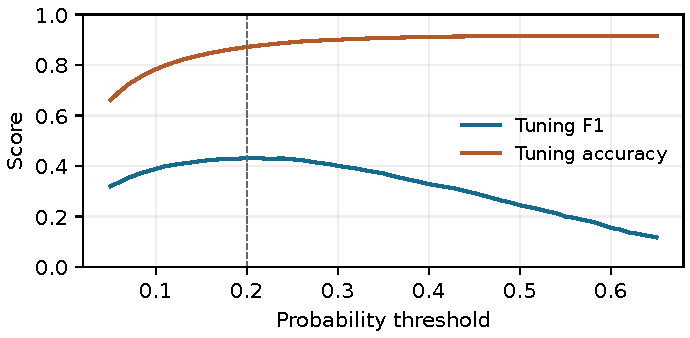
\includegraphics[width=\columnwidth]{figures/threshold_tradeoff.pdf}
\caption{Tuning scores for the selected logistic model. The dashed line marks
the tuning-selected threshold; no holdout labels determine this choice.}
\label{fig:threshold}
\end{figure}

Three-fold CV on the non-holdout pool yields F1 \CVMean{} $\pm$ \CVStd{}
(sample standard deviation). Each fold refits processing and calibrates its
threshold inside the outer training partition. Family selection is not nested,
so this is a consistency diagnostic. A conditional IID-row bootstrap interval
for holdout F1 is [0.4125, 0.4321]; it ignores survey design and selection
variability and is not a population-level clinical interval.

\section{Limitations and reproduction}
Survey nonresponse, optional modules, self-report and shared sampling structure
limit interpretation. False negatives remain substantial (45.54\% of positives),
and a recall-oriented threshold introduces many false positives. We did not
establish prospective validity, fairness across populations, full semantic
cleaning, or coefficient-wise stability. Small ablation gains are not established
as significant or consistent across folds; only the selected configuration has
the three-fold diagnostic. The 120-step final fit also stops before convergence.

After freezing choices, we refit processing and weights on all labeled rows,
producing 1,183 design columns because the larger fit discovers more categories.
\texttt{run.py} loads the saved weights and fitted transformations; seed 433 and
threshold 0.20 reproduce the CSV. From the repository root, run
\texttt{python run.py} with \texttt{--data-dir dataset},
\texttt{--output new.csv}, and \texttt{--seed 433}. Two executions, including
a fresh source directory and CSV cache, produce identical SHA-256 hashes in the
same Python 3.12.14 / NumPy 2.5.3 environment. Cross-backend bitwise identity is
unverified. Training code, indices, configurations, source/data fingerprints and
measurements are saved. No AIcrowd acceptance or score is claimed.

\textbf{Unresolved:} public GitHub commit permalink, staff AI-use
policy and metric clarification. The requester authorized AI assistance;
independent course-policy verification remains pending. All students must review
the generated code and text before submission.

\clearpage
\begin{thebibliography}{3}
\bibitem{cdc} CDC, ``2015 BRFSS Codebook and Calculated Variables,'' 2016--2017.
\url{https://www.cdc.gov/brfss/annual_data/annual_2015.html}.
\bibitem{rules} AIcrowd, ``EPFL Machine Learning Project 1: Challenge Rules,''
accessed Oct. 29, 2026.
\url{https://www.aicrowd.com/challenges/epfl-machine-learning-project-1/challenge_rules}.
\bibitem{leaderboard} AIcrowd, ``EPFL Machine Learning Project 1: Leaderboard,''
accessed Oct. 29, 2026.
\url{https://www.aicrowd.com/challenges/epfl-machine-learning-project-1/leaderboards}.
\end{thebibliography}
\end{document}
